\documentclass[11pt,aspectratio=169]{beamer}
\usepackage{latexsym}
\usepackage{epsfig}
\usepackage{times}
\usepackage{enumerate}
\usepackage{bm}
\usepackage{tikz}
\usepackage{amsthm, amsmath,amsfonts, amssymb}
\usepackage{algorithm,algorithmic}
\usepackage{tikz-network}
\usepackage{color}
\usepackage{setspace}
\usepackage{color}

\definecolor{lightblue}{RGB}{171, 215, 230}

\usetheme{Copenhagen}
\setbeamertemplate{navigation symbols}{}
\setbeamercovered{transparent}
\setbeamertemplate{itemize items}[default]
\setbeamertemplate{enumerate items}[default]

\title{Connection Game}
\author{Nuo Xu}
\institute{Technical University of Munich}
\date{15.11.2024}

\begin{document}
\frame{\titlepage}
\onehalfspacing
\begin{frame}{Classic Steiner Tree Problem}
    Given an undirected graph \(G = (V,E)\) with non-negative edge cost \(c_e \geq 0\) for every edge $c_e \in E$.\\
    \vspace{10pt}
    In the Steiner Tree problem, we are given a set of terminals $R \subseteq V $. The goal is to compute the minimum-cost subgraph that spans all terminals. 
\end{frame}
\begin{frame}{Steiner Tree with Two Terminals}
    If $|R| = 2$, then it is equal to find the shortest path between two terminals.\\
    \vspace{20pt}
    \centering
    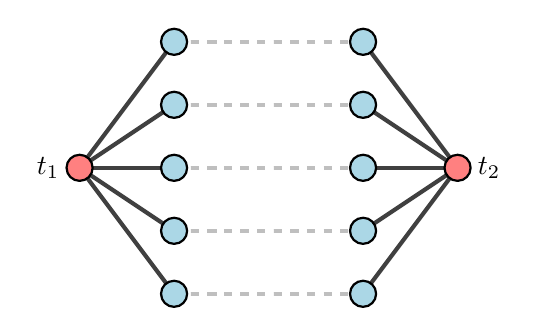
\begin{tikzpicture}[scale =0.8]
        \coordinate (t1) at (-3,0);
        \coordinate (t2) at (3,0);
        \coordinate (l1) at (-1.5,2);
        \coordinate (l2) at (-1.5,1);
        \coordinate (l3) at (-1.5,0);
        \coordinate (l4) at (-1.5,-1);
        \coordinate (l5) at (-1.5,-2);

        \coordinate (r1) at (1.5,2);
        \coordinate (r2) at (1.5,1);
        \coordinate (r3) at (1.5,0);
        \coordinate (r4) at (1.5,-1);
        \coordinate (r5) at (1.5,-2);

        \node[draw,circle,fill=red!50,thick,minimum size=8pt] (CircleNode) at (t1){};
        \node at (-3.5,0) {$t_1$};
        \node at (3.5,0) {$t_2$};
        \node[draw,circle,fill=red!50,thick,minimum size=8pt] (CircleNode) at (t2){};
        \node[draw,circle,fill=lightblue,thick,minimum size=8pt] (CircleNode) at (l1){};
        \node[draw,circle,fill=lightblue,thick,minimum size=8pt] (CircleNode) at (l2){};
        \node[draw,circle,fill=lightblue,thick,minimum size=8pt] (CircleNode) at (l3){};
        \node[draw,circle,fill=lightblue,thick,minimum size=8pt] (CircleNode) at (l4){};
        \node[draw,circle,fill=lightblue,thick,minimum size=8pt] (CircleNode) at (l5){};
        \node[draw,circle,fill=lightblue,thick,minimum size=8pt] (CircleNode) at (r1){};
        \node[draw,circle,fill=lightblue,thick,minimum size=8pt] (CircleNode) at (r2){};
        \node[draw,circle,fill=lightblue,thick,minimum size=8pt] (CircleNode) at (r3){};
        \node[draw,circle,fill=lightblue,thick,minimum size=8pt] (CircleNode) at (r4){};
        \node[draw,circle,fill=lightblue,thick,minimum size=8pt] (CircleNode) at (r5){};
        \Edge(t1)(l1)
        \Edge(t1)(l2)
        \Edge(t1)(l3)
        \Edge(t1)(l4)
        \Edge(t1)(l5)
        \Edge(t2)(r1)
        \Edge(t2)(r2)
        \Edge(t2)(r3)
        \Edge(t2)(r4)
        \Edge(t2)(r5)
        \Edge[style={dashed},color=gray!50](l1)(r1)
        \Edge[style={dashed},color=gray!50](l2)(r2)
        \Edge[style={dashed},color=gray!50](l3)(r3)
        \Edge[style={dashed},color=gray!50](l4)(r4)
        \Edge[style={dashed},color=gray!50](l5)(r5)
    \end{tikzpicture}
     \vspace{20pt}
     
     Dijkstra's algorithm can find the shortest path  polynomial time.
\end{frame}

\begin{frame}{Steiner Tree with N Terminals}
If $|R| = |V|$, then is is equal to find the MST.\\
\vspace{20pt}
    \centering
    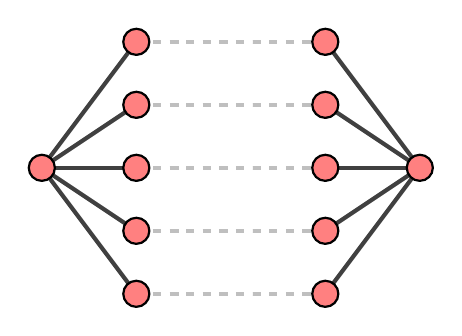
\begin{tikzpicture}[scale =0.8]
        \coordinate (t1) at (-3,0);
        \coordinate (t2) at (3,0);
        \coordinate (l1) at (-1.5,2);
        \coordinate (l2) at (-1.5,1);
        \coordinate (l3) at (-1.5,0);
        \coordinate (l4) at (-1.5,-1);
        \coordinate (l5) at (-1.5,-2);

        \coordinate (r1) at (1.5,2);
        \coordinate (r2) at (1.5,1);
        \coordinate (r3) at (1.5,0);
        \coordinate (r4) at (1.5,-1);
        \coordinate (r5) at (1.5,-2);

        \node[draw,circle,fill=red!50,thick,minimum size=8pt] (CircleNode) at (t1){};
        \node[draw,circle,fill=red!50,thick,minimum size=8pt] (CircleNode) at (t2){};
        \node[draw,circle,fill=red!50,thick,minimum size=8pt] (CircleNode) at (l1){};
        \node[draw,circle,fill=red!50,thick,minimum size=8pt] (CircleNode) at (l2){};
        \node[draw,circle,fill=red!50,thick,minimum size=8pt] (CircleNode) at (l3){};
        \node[draw,circle,fill=red!50,thick,minimum size=8pt] (CircleNode) at (l4){};
        \node[draw,circle,fill=red!50,thick,minimum size=8pt] (CircleNode) at (l5){};
        \node[draw,circle,fill=red!50,thick,minimum size=8pt] (CircleNode) at (r1){};
        \node[draw,circle,fill=red!50,thick,minimum size=8pt] (CircleNode) at (r2){};
        \node[draw,circle,fill=red!50,thick,minimum size=8pt] (CircleNode) at (r3){};
        \node[draw,circle,fill=red!50,thick,minimum size=8pt] (CircleNode) at (r4){};
        \node[draw,circle,fill=red!50,thick,minimum size=8pt] (CircleNode) at (r5){};
        \Edge(t1)(l1)
        \Edge(t1)(l2)
        \Edge(t1)(l3)
        \Edge(t1)(l4)
        \Edge(t1)(l5)
        \Edge(t2)(r1)
        \Edge(t2)(r2)
        \Edge(t2)(r3)
        \Edge(t2)(r4)
        \Edge(t2)(r5)
        \Edge[style={dashed},color=gray!50](l1)(r1)
        \Edge[style={dashed},color=gray!50](l2)(r2)
        \Edge[style={dashed},color=gray!50](l3)(r3)
        \Edge[style={dashed},color=gray!50](l4)(r4)
        \Edge[style={dashed},color=gray!50](l5)(r5)
    \end{tikzpicture}
     \vspace{20pt}
     
     Prim's algorithm can find the minimum spanning tree  polynomial time.
\end{frame}

\begin{frame}{Steiner Tree Example}
    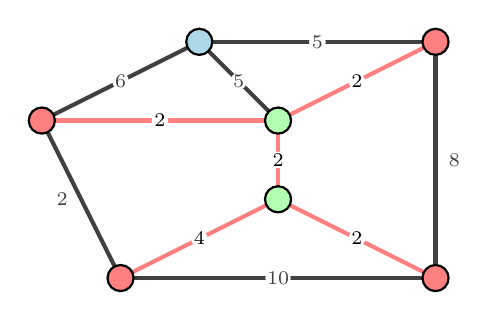
\begin{tikzpicture}
        \coordinate (v1) at (0,0);
        \coordinate (v2) at (3,0);
        \coordinate (v3) at (1,-1);
        \coordinate (v4) at (-2,-1);
		\coordinate (v5) at (-1,-3);
		\coordinate (v6) at (1,-2);
		\coordinate (v7) at (3,-3);

        \node[draw,circle,fill=lightblue,thick,minimum size=8pt] (CircleNode) at (v1){};
		\node[draw,circle,fill=red!50,thick,minimum size=8pt] (CircleNode) at (v2){};
		\node[draw,circle,fill=green!30,thick,minimum size=8pt] (CircleNode) at (v3){};
		\node[draw,circle,fill=red!50,thick,minimum size=8pt] (CircleNode) at (v4){};
		\node[draw,circle,fill=red!50,thick,minimum size=8pt] (CircleNode) at (v5){};
		\node[draw,circle,fill=green!30,thick,minimum size=8pt] (CircleNode) at (v6){};
        \node[draw,circle,fill=red!50,thick,minimum size=8pt] (CircleNode) at (v7){};

        \Edge[label=$5$](v1)(v2)
        \Edge[label=$5$](v1)(v3)
        \Edge[label=$6$](v1)(v4)
        \Edge[label=$2$,color=red!50,fontcolor=black](v2)(v3)
        \Edge[label=$2$,position={left=1mm}](v4)(v5)
        \Edge[label=$2$,color=red!50,fontcolor=black](v4)(v3)
        \Edge[label=$2$,color=red!50,fontcolor=black](v3)(v6)
        \Edge[label=$4$,color=red!50,fontcolor=black](v5)(v6)
        \Edge[label=$10$](v5)(v7)
        \Edge[label=$8$,position={right=1mm}](v2)(v7)
        \Edge[label=$2$,color=red!50,fontcolor=black,](v6)(v7)     
    \end{tikzpicture}\hspace{10pt}
    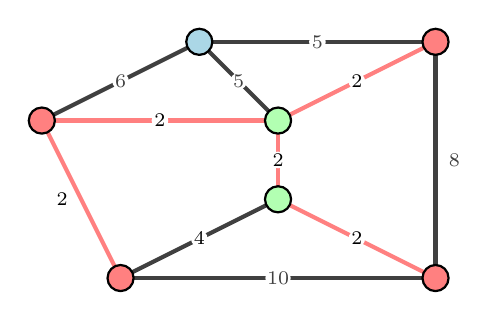
\begin{tikzpicture}
        \coordinate (v1) at (0,0);
        \coordinate (v2) at (3,0);
        \coordinate (v3) at (1,-1);
        \coordinate (v4) at (-2,-1);
		\coordinate (v5) at (-1,-3);
		\coordinate (v6) at (1,-2);
		\coordinate (v7) at (3,-3);

        \node[draw,circle,fill=lightblue,thick,minimum size=8pt] (CircleNode) at (v1){};
		\node[draw,circle,fill=red!50,thick,minimum size=8pt] (CircleNode) at (v2){};
		\node[draw,circle,fill=green!30,thick,minimum size=8pt] (CircleNode) at (v3){};
		\node[draw,circle,fill=red!50,thick,minimum size=8pt] (CircleNode) at (v4){};
		\node[draw,circle,fill=red!50,thick,minimum size=8pt] (CircleNode) at (v5){};
		\node[draw,circle,fill=green!30,thick,minimum size=8pt] (CircleNode) at (v6){};
        \node[draw,circle,fill=red!50,thick,minimum size=8pt] (CircleNode) at (v7){};

        \Edge[label=$5$](v1)(v2)
        \Edge[label=$5$](v1)(v3)
        \Edge[label=$6$](v1)(v4)
        \Edge[label=$2$,color=red!50,fontcolor=black](v2)(v3)
        \Edge[label=$2$,color=red!50,fontcolor=black,position={left=1mm}](v4)(v5)
        \Edge[label=$2$,color=red!50,fontcolor=black](v4)(v3)
        \Edge[label=$2$,color=red!50,fontcolor=black](v3)(v6)
        \Edge[label=$4$,fontcolor=black](v5)(v6)
        \Edge[label=$10$](v5)(v7)
        \Edge[label=$8$,position={right=1mm}](v2)(v7)
        \Edge[label=$2$,color=red!50,fontcolor=black](v6)(v7)     
    \end{tikzpicture}
\end{frame}

\begin{frame}{Steiner Forest Problem}
 Given a collection of disjoint subsets of \(V: V_1,V_2,V_3,...V_n\). The goal is to compute a subgraph that any two vertices that belong to the same subset \(V_i\) are connected.
\end{frame}

\begin{frame}{Introduction of Selfish Agents}
However, when players start to have self-interests, some players might need to pay more if they choose to discard self-interests to archive best centralized optimum. \\
\vspace{10pt}
Given an undirected graph \(G\) with non-negative edge costs and \(N\) players, each player is interested in connecting a set of terminals (nodes in \(G\)) via buying a subgraph of \(G\). \\
\vspace{10pt}
Players offer each edge in \(G\) certain amount of money, and they would like to pay a little as possible. 
\end{frame}

\begin{frame}{How Selfish Agents Cause Deviation from Central OPT}
    \begin{figure}
        \begin{center}
    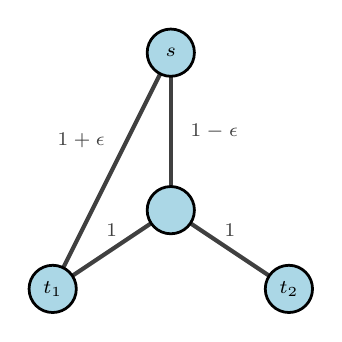
\begin{tikzpicture}
	\Vertex[label=$t_1$]{t1}
	\Vertex[label=$t_2$,x=3]{t2}
	\Vertex[x=1.5,y=1]{middle}
	\Vertex[x=1.5,y=3,label=$s$]{s}
	\Edge[label=$1$,position={above=1mm}](t1)(middle)
	\Edge[label=$1$,position={above=1mm}](t2)(middle)
	\Edge[label=$1-\epsilon$,position={right = 2mm}](s)(middle)
	\Edge[label=$1+\epsilon$,position={above left=2mm}](t1)(s)
\end{tikzpicture}
\hspace*{10pt}
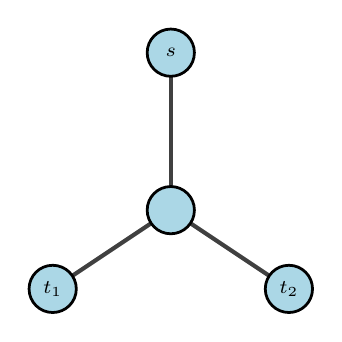
\begin{tikzpicture}
	\Vertex[label=$t_1$]{t1}
	\Vertex[label=$t_2$,x=3]{t2}
	\Vertex[x=1.5,y=1]{middle}
	\Vertex[x=1.5,y=3,label=$s$]{s}
	\Edge(t1)(middle)
	\Edge(t2)(middle)
	\Edge(s)(middle)
\end{tikzpicture}
\hspace*{10pt}
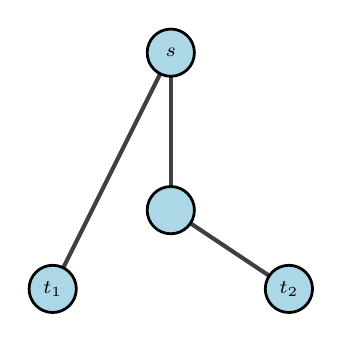
\begin{tikzpicture}
	\Vertex[label=$t_1$]{t1}
	\Vertex[label=$t_2$,x=3]{t2}
	\Vertex[x=1.5,y=1]{middle}
	\Vertex[x=1.5,y=3,label=$s$]{s}
	\Edge(t2)(middle)
	\Edge(s)(middle)
	\Edge(t1)(s)
\end{tikzpicture}
    
\end{center}
\end{figure}
\end{frame}


\begin{frame}{Formal Definition of Connection Game}
    \begin{definition}[Connection Game]
          \begin{itemize}
            \item An undirected graph \(G = (V,E)\).
            \item Non-negative edge cost \(c_e \geq 0\) for every edge $c_e \in E$.
            \item A subset of \(V\) for each player that they must connect to. 
            \item A payment function \(p_i\) indicates that player's payment strategy. \(p_i(e)\) is the contribution that player \(i\) would like to offer for edge \(e\).
    \end{itemize}
    \end{definition}
\end{frame}

\begin{frame}{Rules of Connection Game}
\begin{definition}[Connection Game]
    \begin{itemize}
    \item If the sum of payment on certain edge \(e\) is larger than the cost on that edge \(c_e\), this edge is considered as bought.
    \item If an edge is bought, it can be used by all players no matter they contribute to it or not. \\
    \item The goal of all players is to connect all of their terminals. If in the end, a player's terminates are not fully connected, they will face an infinite penalty.  
    \end{itemize}
    \end{definition}
\end{frame}

\begin{frame}{Nash's Theorem}
   
    \begin{theorem}[Nash's theorem]
        With randomization, any game with finite number of players and actions has a mixed-strategy of Nash equilibrium.
    \end{theorem}
    Nash's theorem states that any finite game has at least one mixed strategies Nash equilibrium but no grantee on pure strategy equilibrium.  
\end{frame}

\begin{frame}{Nash Equilibrium in Coonection Game}
     \begin{definition}[Nash Equilibrium in Connection Game]
        A Nash equilibrium of the connection game is a payment function p such that, if players offer payments \(p\), no payer has an incentive to deviate from their payment. 
    \end{definition}
    \textbf{Pure Nash equilibrium may not exist in the connection game.}
\end{frame}

\begin{frame}{No Existence of Nash Equilibrium}
\centering
    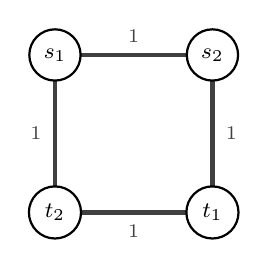
\begin{tikzpicture}
        \coordinate (s1) at (0,0);
        \coordinate (s2) at (2,0);
        \coordinate (t2) at (0,-2);
        \coordinate (t1) at (2,-2);

        \node[draw,circle,fill=white,thick,minimum size=2pt] (CircleNode) at (s1){\footnotesize $s_1$};
        \node[draw,circle,fill=white,thick,minimum size=2pt] (CircleNode) at (s2){\footnotesize $s_2$};
        \node[draw,circle,fill=white,thick,minimum size=2pt] (CircleNode) at (t1){\footnotesize $t_1$};
        \node[draw,circle,fill=white,thick,minimum size=2pt] (CircleNode) at (t2){\footnotesize $t_2$};

        \Edge[label=$1$,position={above=1mm}](s1)(s2)
        \Edge[label=$1$,position={right=1mm}](s2)(t1)
        \Edge[label=$1$,position={below=1mm}](t1)(t2)
        \Edge[label=$1$,position={left=1mm}](t2)(s1)
    \end{tikzpicture}
    \hspace{10pt}
    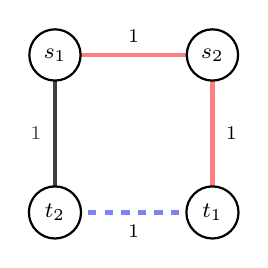
\begin{tikzpicture}
        \coordinate (s1) at (0,0);
        \coordinate (s2) at (2,0);
        \coordinate (t2) at (0,-2);
        \coordinate (t1) at (2,-2);

        \node[draw,circle,fill=white,thick,minimum size=2pt] (CircleNode) at (s1){\footnotesize  $s_1$};
        \node[draw,circle,fill=white,thick,minimum size=2pt] (CircleNode) at (s2){\footnotesize $s_2$};
        \node[draw,circle,fill=white,thick,minimum size=2pt] (CircleNode) at (t1){\footnotesize $t_1$};
        \node[draw,circle,fill=white,thick,minimum size=2pt] (CircleNode) at (t2){\footnotesize $t_2$};

        \Edge[label=$1$,fontcolor=black,color=red!50,position={above=1mm}](s1)(s2)
        \Edge[label=$1$,fontcolor=black,color=red!50,position={right=1mm}](s2)(t1)
        \Edge[label=$1$,fontcolor=black,color=blue!50,style={dashed},position={below=1mm}](t1)(t2)
        \Edge[label=$1$,position={left=1mm}](t2)(s1)
    \end{tikzpicture}
    \hspace{10pt}
    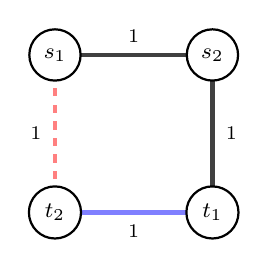
\begin{tikzpicture}
        \coordinate (s1) at (0,0);
        \coordinate (s2) at (2,0);
        \coordinate (t2) at (0,-2);
        \coordinate (t1) at (2,-2);

        \node[draw,circle,fill=white,thick,minimum size=2pt] (CircleNode) at (s1){\footnotesize $s_1$};
        \node[draw,circle,fill=white,thick,minimum size=2pt] (CircleNode) at (s2){\footnotesize $s_2$};
        \node[draw,circle,fill=white,thick,minimum size=2pt] (CircleNode) at (t1){\footnotesize $t_1$};
        \node[draw,circle,fill=white,thick,minimum size=2pt] (CircleNode) at (t2){\footnotesize $t_2$};

        \Edge[label=$1$,fontcolor=black,position={above=1mm}](s1)(s2)
        \Edge[label=$1$,fontcolor=black,position={right=1mm}](s2)(t1)
        \Edge[label=$1$,fontcolor=black,color=blue!50,position={below=1mm}](t1)(t2)
        \Edge[label=$1$,fontcolor=black,color=red!50,style={dashed},position={left=1mm}](t2)(s1)
    \end{tikzpicture}    
\end{frame}

\begin{frame}{Fractional Nash Equilibrium}
\begin{definition}[Fractional Nash Equilibrium]
    Game instances where the only Nash equilibria in existence require players to split the cost of an edge. 
\end{definition}
\vspace{10pt}
\centering
 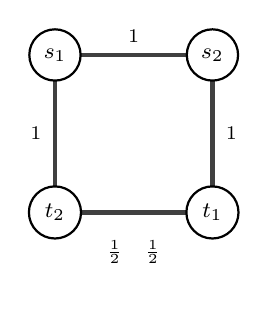
\begin{tikzpicture}
        \coordinate (s1) at (0,0);
        \coordinate (s2) at (2,0);
        \coordinate (t2) at (0,-2);
        \coordinate (t1) at (2,-2);

        \node[draw,circle,fill=white,thick,minimum size=2pt] (CircleNode) at (s1){\footnotesize $s_1$};
        \node[draw,circle,fill=white,thick,minimum size=2pt] (CircleNode) at (s2){\footnotesize $s_2$};
        \node[draw,circle,fill=white,thick,minimum size=2pt] (CircleNode) at (t1){\footnotesize $t_1$};
        \node[draw,circle,fill=white,thick,minimum size=2pt] (CircleNode) at (t2){\footnotesize $t_2$};

        \Edge[label=$1$,fontcolor=black,position={above=1mm}](s1)(s2)
        \Edge[label=$1$,fontcolor=black,position={right=1mm}](s2)(t1)
        \Edge[label=$\frac{1}{2}\quad\frac{1}{2}$,fontcolor=black,position={below=1mm}](t1)(t2)
        \Edge[label=$1$,fontcolor=black,position={left=1mm}](t2)(s1)
    \end{tikzpicture} 
\end{frame}

\begin{frame}{Some Properties of Nash Equilibrium}
    \begin{itemize}
        \item \(G_p\) is a forest.
        \item Let \(T^i\) be the smallest tree in \(G_p\) connecting all terminals of player \(i\), then player \(i\) only contributes to edges in \(T^i\).
        \item Each edge is either bought or not at all. 
    \end{itemize}
    
\end{frame}

\begin{frame}{Price of Anarchy}
    As shown before, the introduction of selfish agents can lead to worse equilibrium than the best centralized optimum. The question is how bad an equilibrium can be.

    \begin{definition}[Price of Anarchy] The price of anarchy of connection game is defined as the ratio of the cost of worst Nash equilibrium over the best centralized design.
        \[P_A = \dfrac{\sum_{1}^{N}p_i(e) }{OPT}\]
    \end{definition}
   
\end{frame}

\begin{frame}{Price of Anarchy}
    \begin{lemma}
        The Price of Anarchy in connection game can be as bad as \(N\).
    \end{lemma}
\end{frame}

\begin{frame}{Price of Stability}
    Price of stability is a complementary concept of price of anarchy which evaluate how good the best equilibrium can be. 

\begin{definition}[Price of Stability] 
    The price of anarchy of connection game is defined as the ratio of the cost of best Nash equilibrium over the best centralized design.
    \[P_A = \dfrac{\sum_{1}^{N}p_i(e) }{OPT}\]
    \end{definition}
\end{frame}

\begin{frame}{Single Source Game}
    In the single source game, we only allow every player \(i\) has one unique terminal \(t_i\) that they all would like to connect a common terminal \(s\). This can be considered as a special version of Steiner tree problem where \(R = \{s,t_1,t_2,...,t_n\}\). 
\vspace{10pt}
\begin{definition}[Single source Game]
	A single source game is a game in which all players share a common terminal \(s\) and in addition, each player \(i\) has exactly one other terminal \(t_i\).
\end{definition}
\end{frame}

\begin{frame}{Suppose We have $T^*$ in our hands \dots}
Now suppose the minimum cost Steiner tree \(T^*\) over all players' terminals is given on a sliver plate, one natural thought is can we achieve an equilibrium that equals to the \(OPT\)?  \\
\vspace{10pt}
The answer is YES!
\end{frame}

\begin{frame}{A Not Important Property of $T^*$}
    It is trivial to see that every leaf node in \(T^*\) is a terminal as if not it is possible to simply discard this node and corresponding edge without affecting the connection of any terminals.
    \vspace{10pt}
\begin{fact}
	Every leaf node in \(T^*\) is a terminal. 
\end{fact}
\end{frame}

\begin{frame}{How Should We Traverse $T^*$?}
\begin{columns}
    \column{0.7\textwidth}
    First, let \(T^*\) be rooted from \(s\). \\
    \vspace{10pt}
    For every edge \(e\), suppose \(e\) is removed from \(T^*\), \(T^*\) will be divided into two subtrees.\\
    \vspace{10pt}
    Let the subtree that does not contain \(s\) be \(T_e\) and the one contains \(s\) be \(T_s\).\\
    \vspace{10pt}
    \textbf{We will visit \(T^*\) in reverse breadth-first-search order.\\}
    \column{0.3\textwidth}
    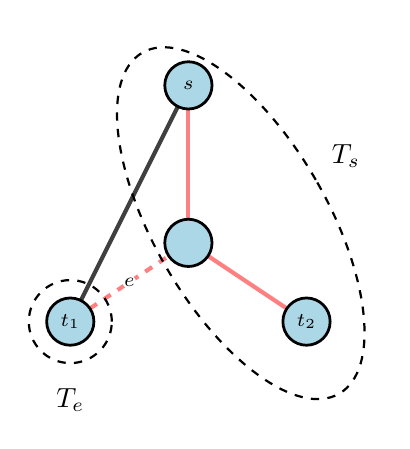
\begin{tikzpicture}
			\Vertex[label=$t_1$]{t1}
			\Vertex[label=$t_2$,x=3]{t2}
			\Vertex[x=1.5,y=1]{middle}
			\Vertex[x=1.5,y=3,label=$s$]{s}
			\Edge[style={dashed},label=$e$,color=red!50,fontcolor=black](t1)(middle)
			\Edge[color=red!50](t2)(middle)
			\Edge[color=red!50](s)(middle)
			\Edge(t1)(s)
			\draw[dashed,thick](0,0) circle (15pt);
			\node at (0, -1) {$T_e$};
			\draw[dashed,thick,rotate=30,label=$T_s$](2.5,0) ellipse(1.1cm and 2.5cm);
 		\node at (3.5, 2.1) {$T_s$};
		\end{tikzpicture}
\end{columns}
\end{frame}

\begin{frame}{How to Assign \(p_i(e)\)?}
In every iteration, we modify the cost of every edge according to the following rules:
\begin{itemize}
	\item let costs of edges \(e \in T_e\) be \(p_i(e)\)
	\item let costs of edges \(e \in T_s\) be  0
	\item costs of edges \(e\notin T^*\) stay the the same
\end{itemize}
\vspace{10pt}
\end{frame}

\begin{frame}{How to Assign \(p_i(e)\)?}
    We can find the cheapest alternative path \(A_i\) from \(t_i\) to \(s\) from \(G \setminus \{e\}\) under modified cost in polynomial time. \\
    \vspace{10pt}
    Find the minimum value of:
    \begin{itemize}
        \item $c(e) - $ contribution from other players to edge \(e\)
        \item cost of \(A_i-\) sum of all contribution of player \(i\) to \(T^*\) 
    \end{itemize}
\end{frame}

\begin{frame}{Algorithm}
\begin{algorithm}[H]
\begin{algorithmic}[1]
    \STATE $p_i(e) \gets 0, \forall t_i \in R, \forall e \in E$ 
    \WHILE{$e \in ReverseBFS(T^*)$}
    \IF{$e$ is a cut} 
    \STATE $p_i(e) \gets c(e)$
    \ELSE
    \STATE \(c(e) \gets p_i(f)  \qquad \forall e \in T_e\) 
	\STATE \(c(e) \gets 0 \qquad \forall e \in T_S\) 
    \STATE $A_i \gets$ cheapest alternative path from \(s\) to \(t_i\) in $G\setminus\{e\}$ 
    \STATE \(p_i(e) \gets min\{c(A_i) - \sum_{e\in T^*}p_i(e),c(e)-\sum_{j}p_j(e) \}\)
    \ENDIF
    \ENDWHILE
\end{algorithmic}
\caption{pseudocode for assigning $p_i(e)$ }
\label{alg:seq}
\end{algorithm}
\end{frame}

\begin{frame}{Example}
\begin{columns}
    \column{0.5\textwidth}
    \centering
 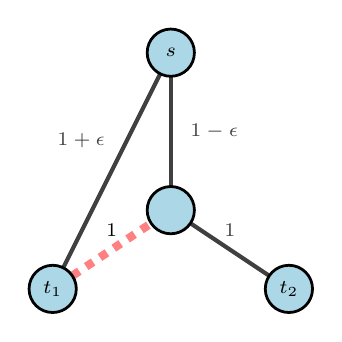
\begin{tikzpicture}
	\Vertex[label=$t_1$]{t1}
	\Vertex[label=$t_2$,x=3]{t2}
	\Vertex[x=1.5,y=1]{middle}
	\Vertex[x=1.5,y=3,label=$s$]{s}
	\Edge[label=$1$,style={dashed},fontcolor=black, color=red!50,position={above=1mm},lw=3pt](t1)(middle)
	\Edge[label=$1$,position={above=1mm}](t2)(middle)
	\Edge[label=$1-\epsilon$,position={right = 2mm}](s)(middle)
	\Edge[label=$1+\epsilon$,position={above left=2mm}](t1)(s)
\end{tikzpicture}
\column{0.5\textwidth}
\doublespacing
$e$ is not a cut.\\
consider $c(A_1) = 1+\epsilon, \quad p_1(T^*) = 0$\\
$c(e) = 1, \quad  \sum_{j}p_j(e) = 0$\\
set $p_1(e) = 1$
\end{columns}
\end{frame}

\begin{frame}{Example}
\begin{columns}
    \column{0.5\textwidth}
    \centering
 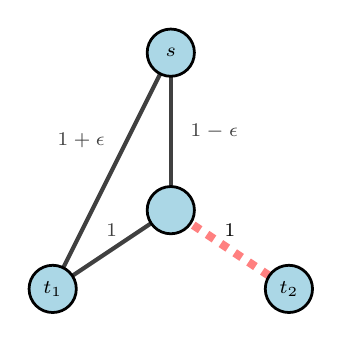
\begin{tikzpicture}
	\Vertex[label=$t_1$]{t1}
	\Vertex[label=$t_2$,x=3]{t2}
	\Vertex[x=1.5,y=1]{middle}
	\Vertex[x=1.5,y=3,label=$s$]{s}
	\Edge[label=$1$,position={above=1mm}](t1)(middle)
	\Edge[label=$1$,,style={dashed},fontcolor=black,lw=3pt,color=red!50,position={above=1mm}](t2)(middle)
	\Edge[label=$1-\epsilon$,position={right = 2mm}](s)(middle)
	\Edge[label=$1+\epsilon$,position={above left=2mm}](t1)(s)
\end{tikzpicture}
\column{0.5\textwidth}
\doublespacing
$e$ is a cut.\\
set $p_2(e) = 1$
\end{columns}
\end{frame}

\begin{frame}{Example}
\begin{columns}
    \column{0.5\textwidth}
    \centering
 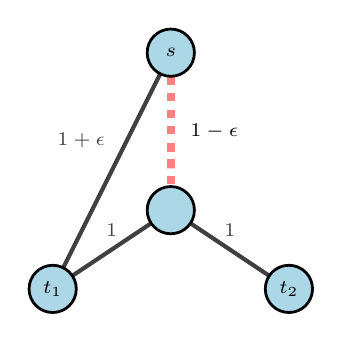
\begin{tikzpicture}
	\Vertex[label=$t_1$]{t1}
	\Vertex[label=$t_2$,x=3]{t2}
	\Vertex[x=1.5,y=1]{middle}
	\Vertex[x=1.5,y=3,label=$s$]{s}
	\Edge[label=$1$,position={above=1mm}](t1)(middle)
	\Edge[label=$1$,position={above=1mm}](t2)(middle)
	\Edge[label=$1-\epsilon$,,style={dashed},fontcolor=black,lw=3pt,color=red!50,position={right = 2mm}](s)(middle)
	\Edge[label=$1+\epsilon$,position={above left=2mm}](t1)(s)
\end{tikzpicture}
\column{0.5\textwidth}
\doublespacing
$e$ is not a cut.\\
\textbf{for $t_1$}\\
$c(A_1) = 1+\epsilon, \quad  p_1(T^*) = 1$\\
$c(e) = 1-\epsilon, \quad \sum_{j}p_j(e) = 0$\\
set $p_1(e) = \epsilon$\\
\textbf{for $t_2$}\\
$c(A_2) = 3+\epsilon, \quad p_2(T^*) = 1$\\
$c(e) = 1-\epsilon,\quad  \sum_{j}p_j(e) = \epsilon$\\
set $p_2(e) = 1-2\epsilon$
\end{columns}
\end{frame}


\begin{frame}{Proof of \(p\) Being Nash Equilibrium}
\begin{corollary}
	The final payment function produced by the above algorithm is indeed a Nash equilibrium.
\end{corollary}
\vspace{10pt}
By assigning $p_i(e) = min\{c(A_i) - \sum_{e\in T^*}p_i(T^*), c(e) - \sum_{j\in T_i,j\neq i}p_j(e)\}$, we ensure that player \(i\) will never contribute to \(e\) more than the cost of deviation. \\
\vspace{10pt}
In another word, it is never player $i$'s interests to deviate from buying $e$. And this holds true for every player in every edge in $T^*$. Therefore, \(p\) is indeed a Nash equilibrium. 

\end{frame}

\begin{frame}{Proof of Price of Stability Being 1}
To prove that the price of stability is always 1, we need to demonstrate that in the end of the game, every edge in \(T^*\) is fully paid. 
\end{frame}

\begin{frame}{Proof Agenda}
First, we are going to assume that the following lemma is true. 
\vspace{10pt}\\
Suppose \(A_i\) is \(i\)'s alternative path at some stage of the algorithm. Then suppose there are two nodes \(v\) and \(w\) on \(A_i\) that divides this path into three parts. Let edges on \(A_i\) from \(t_i\) to \(v\) be \(f_1\), from \(v\) to \(w\) be \(f_2\), from \(w\) to \(s\) be \(f_3\).
\vspace{10pt}
\begin{lemma}
	There must exist a pair of \(\{v,w\}\) such that \(f_1 \in T_e\), \(f_2 \notin T^*\), \(f_3 \in T^*\setminus T_e\).
\end{lemma}
\vspace{10pt}
Once \(A_i\) leaves \(T_e\), it will never go back to \(T_e\) again.
\end{frame}

\begin{frame}{Proof via Contradiction}
\begin{lemma}
	All edges in \(T^*\) are bought, i.e. $\sum p_i(e) = c(e)$ for any $e \in T^*$.
\end{lemma}

Suppose there exists some edge \(e\) such that after all players in \(T_e\) have contributed to that edge, \(p_i(e) < c(e)\), we can prove that \(T_e\) costs more than \(\bigcup_{i\in T_e} A_i\) which is a contradiction of \(T^*\) is \(OPT\).
\end{frame}

\begin{frame}{Approximate Nash Equilibrium}
    Although we proved that the determined existence of Nash equilibrium in single source game, \textbf{the algorithm presented is not feasible} as the finding the minimum cost Steiner tree is NP-hard by itself. \\
    \vspace{10pt}
\begin{definition}[Approximate Equilibrium]
	A \((1+\epsilon)\)-approximate Nash Equilibrium is a payment function \(p\) such that player \(i\) would not deviate their payment by a factor of \(1+\epsilon\).
\end{definition}
\end{frame}

\begin{frame}{Approximate Nash Equilibrium in Connection Game}
If we are given an approximated Steiner tree \(T\) and try to use the same algorithm to assign \(p_i(e)\) in \(T\), since \(T\) is not optimal, there will be some edge \(e\) that players are unwilling to pay for. \\
\vspace{20pt}
\centering
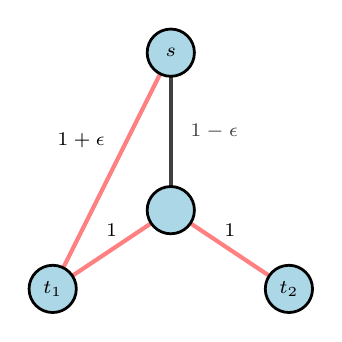
\begin{tikzpicture}
	\Vertex[label=$t_1$]{t1}
	\Vertex[label=$t_2$,x=3]{t2}
	\Vertex[x=1.5,y=1]{middle}
	\Vertex[x=1.5,y=3,label=$s$]{s}
	\Edge[label=$1$,fontcolor=black,color=red!50,position={above=1mm}](t1)(middle)
	\Edge[label=$1$,fontcolor=black,color=red!50,position={above=1mm}](t2)(middle)
	\Edge[label=$1-\epsilon$,position={right = 2mm}](s)(middle)
    \Edge[label=$1+\epsilon$,fontcolor=black,color=red!50,position={above left=2mm}](t1)(s)
\end{tikzpicture}
\end{frame}

\begin{frame}{Example}
\begin{columns}
    \column{0.5\textwidth}
    \centering
 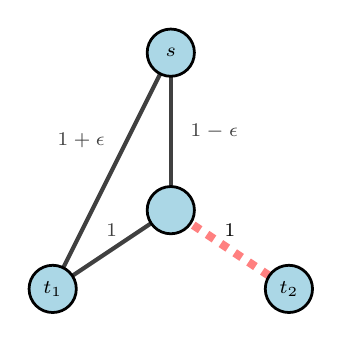
\begin{tikzpicture}
	\Vertex[label=$t_1$]{t1}
	\Vertex[label=$t_2$,x=3]{t2}
	\Vertex[x=1.5,y=1]{middle}
	\Vertex[x=1.5,y=3,label=$s$]{s}
	\Edge[label=$1$,position={above=1mm}](t1)(middle)
	\Edge[label=$1$,style={dashed},fontcolor=black,lw=3pt,color=red!50,position={above=1mm}](t2)(middle)
	\Edge[label=$1-\epsilon$,position={right = 2mm}](s)(middle)
	\Edge[label=$1+\epsilon$,position={above left=2mm}](t1)(s)
\end{tikzpicture}
\column{0.5\textwidth}
\doublespacing
$e$ is a cut.\\
set $p_2(e) = 1$
\end{columns}
\end{frame}

\begin{frame}{Example}
\begin{columns}
    \column{0.5\textwidth}
    \centering
 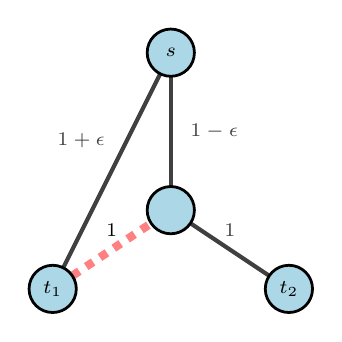
\begin{tikzpicture}
	\Vertex[label=$t_1$]{t1}
	\Vertex[label=$t_2$,x=3]{t2}
	\Vertex[x=1.5,y=1]{middle}
	\Vertex[x=1.5,y=3,label=$s$]{s}
	\Edge[label=$1$,style={dashed},fontcolor=black,lw=3pt,color=red!50,position={above=1mm}](t1)(middle)
	\Edge[label=$1$,position={above=1mm}](t2)(middle)
	\Edge[label=$1-\epsilon$,position={right = 2mm}](s)(middle)
	\Edge[label=$1+\epsilon$,position={above left=2mm}](t1)(s)
\end{tikzpicture}
\column{0.5\textwidth}
\doublespacing
$e$ is not a cut.\\
$c(A_2) = 2-\epsilon,\quad p_2(T^*) =1$\\
$c(e) = 1,\quad \sum_{j}p_j(e) = 0 $\\
set $p_2(e) = 1 - \epsilon$ \\
In the end of the game, $e$ is not fully paid! Player 2 will deviate.
\end{columns}
    
\end{frame}

\begin{frame}{Approximate Nash Equilibrium in Connection Game}
\begin{theorem}
	Given a single source game and \(\alpha\) approximation of minimum-cost Steiner tree \(T\), \(\forall \epsilon > 0\) , there is a polynomial algorithm which return a \((1+\epsilon)\)-approximation \textit{Nash equilibrium} on Steiner Tree \(T^{'}\), where $c(T^{'}) \leq c(T)$.
\end{theorem}
\end{frame}

\begin{frame}{Lower Bound of Approximate Nash Equilibrium}
It has been proven that it is NP-hard to approximate Steiner tree problem within ratio \(96/95\). \\
The closest approximation ratio has been obtained so far is 1.55 by modeling this problem into linear programming and randomized rounding. 
\end{frame}

\begin{frame}{Frame Title}
For any $\epsilon > 0$, there is a game such that any equilibrium which purchases the optimal network is at least a $(3/2-\epsilon)$-approximate Nash equilibrium.
\end{frame}

\end{document}